\documentclass[11pt]{beamer}
\usepackage[utf8]{inputenc}
\usepackage[T1,T2A]{fontenc}
\usepackage[russian]{babel}
\usepackage{color}
\usepackage{listings}
\usepackage{calc}
\usepackage{graphicx}
\usepackage{epstopdf}
\usepackage{hyperref}
\hypersetup{unicode,colorlinks}
\usepackage{csquotes}
\usepackage{upquote}
\usepackage{cprotect}
\usetheme[progressbar=head,numbering=fraction,block=fill]{metropolis}
\usepackage{dejavu}
\usepackage{etoolbox}
\usepackage{bm}
\usepackage{minted}
%\usepackage[defaultsans]{droidsans}
%\usepackage[defaultmono]{droidmono}
%\makeatletter
%\input droid/t1fdm.fd
%\makeatother

\makeatletter
\DeclareRobustCommand*{\bfseries}{%
    \not@math@alphabet\bfseries\mathbf
    \fontseries\bfdefault\selectfont
    \boldmath
}
\makeatother

\makeatletter
\chardef\straightquote@code=\catcode`'
\chardef\backquote@code=\catcode``
\catcode`'=\active \catcode``=\active
\patchcmd{\@noligs}
{\textasciigrave}
{\fixedtextasciigrave}
{}{}
\newcommand{\fixedtextasciigrave}{%
    \makebox[.5em]{\fontencoding{TS1}\fontfamily{fvs}\selectfont\textasciigrave}% Vera Sans
}
\catcode\lq\'=\straightquote@code
\catcode\lq\`=\backquote@code
\makeatletter

\lstset{
    language=Haskell,
    inputencoding=utf8,
    extendedchars=true,
    breaklines=true,
    escapeinside=!!,
    tabsize=4,
    breakatwhitespace=true,
    keepspaces=true,
    basicstyle=\ttfamily,
    commentstyle=\color{gray}\itshape,
    keywordstyle=
    % keywordstyle=\color{blue}, % TODO https://tex.stackexchange.com/questions/415777/avoid-highlighting-keywords-following-certain-words-in-listings
    % addkeywords={Type}
    % deletekeywords={Monad, String, return, array, show},
    % otherkeywords={::, ->}
}
\lstset{
    literate={а}{{\selectfont\char224}}1
    {б}{{\selectfont\char225}}1
    {в}{{\selectfont\char226}}1
    {г}{{\selectfont\char227}}1
    {д}{{\selectfont\char228}}1
    {е}{{\selectfont\char229}}1
    {ё}{{\"e}}1
    {ж}{{\selectfont\char230}}1
    {з}{{\selectfont\char231}}1
    {и}{{\selectfont\char232}}1
    {й}{{\selectfont\char233}}1
    {к}{{\selectfont\char234}}1
    {л}{{\selectfont\char235}}1
    {м}{{\selectfont\char236}}1
    {н}{{\selectfont\char237}}1
    {о}{{\selectfont\char238}}1
    {п}{{\selectfont\char239}}1
    {р}{{\selectfont\char240}}1
    {с}{{\selectfont\char241}}1
    {т}{{\selectfont\char242}}1
    {у}{{\selectfont\char243}}1
    {ф}{{\selectfont\char244}}1
    {х}{{\selectfont\char245}}1
    {ц}{{\selectfont\char246}}1
    {ч}{{\selectfont\char247}}1
    {ш}{{\selectfont\char248}}1
    {щ}{{\selectfont\char249}}1
    {ъ}{{\selectfont\char250}}1
    {ы}{{\selectfont\char251}}1
    {ь}{{\selectfont\char252}}1
    {э}{{\selectfont\char253}}1
    {ю}{{\selectfont\char254}}1
    {я}{{\selectfont\char255}}1
    {А}{{\selectfont\char192}}1
    {Б}{{\selectfont\char193}}1
    {В}{{\selectfont\char194}}1
    {Г}{{\selectfont\char195}}1
    {Д}{{\selectfont\char196}}1
    {Е}{{\selectfont\char197}}1
    {Ё}{{\"E}}1
    {Ж}{{\selectfont\char198}}1
    {З}{{\selectfont\char199}}1
    {И}{{\selectfont\char200}}1
    {Й}{{\selectfont\char201}}1
    {К}{{\selectfont\char202}}1
    {Л}{{\selectfont\char203}}1
    {М}{{\selectfont\char204}}1
    {Н}{{\selectfont\char205}}1
    {О}{{\selectfont\char206}}1
    {П}{{\selectfont\char207}}1
    {Р}{{\selectfont\char208}}1
    {С}{{\selectfont\char209}}1
    {Т}{{\selectfont\char210}}1
    {У}{{\selectfont\char211}}1
    {Ф}{{\selectfont\char212}}1
    {Х}{{\selectfont\char213}}1
    {Ц}{{\selectfont\char214}}1
    {Ч}{{\selectfont\char215}}1
    {Ш}{{\selectfont\char216}}1
    {Щ}{{\selectfont\char217}}1
    {Ъ}{{\selectfont\char218}}1
    {Ы}{{\selectfont\char219}}1
    {Ь}{{\selectfont\char220}}1
    {Э}{{\selectfont\char221}}1
    {Ю}{{\selectfont\char222}}1
    {Я}{{\selectfont\char223}}1
    {`}{{{\fixedtextasciigrave}}}1
}

% \usemintedstyle{solarized-light}
\newminted[haskell]{haskell}{
    escapeinside=``,
    beameroverlays=true,
    texcomments=true,
    autogobble=true,
    fontsize=\small
}
\newmintinline[haskinline]{haskell}{
    escapeinside=``,
    beameroverlays=true,
    texcomments=true
}

\author{Алексей Романов}
\subtitle{Функциональное программирование на Haskell}
%\logo{}
\institute{МИЭТ}
\subject{Функциональное программирование на Haskell}
%\setbeamercovered{transparent}
%\setbeamertemplate{navigation symbols}{}


\title{Лекция 9: ленивость}

\begin{document}
\begin{frame}[plain]
  \maketitle
\end{frame}

\begin{frame}[fragile]
  \frametitle{Передача по значению}
  \begin{itemize}
    \item Как вычисляется выражение вида \haskinline|f(g(x, y), h(z))| в привычных языках?
          \pause
    \item Сначала вычисляются аргументы \haskinline|g(x, y)| и \haskinline|h(z)| (гарантированно в этом порядке или нет), потом их значения передаются в \haskinline|f|.
    \item Это называется \emph{передачей аргументов по значению (call-by-value)}.
    \item Перед вызовом функции вычисляются все её аргументы.
    \item Исключения в C-подобных языках?
          \pause
    \item \haskinline|&&|, \haskinline{||}, \haskinline|? :|.
          \pause
    \item В них вычисляется первый операнд, а второй (и третий для \haskinline|? :|) "--- только если необходимо.
  \end{itemize}
\end{frame}

\begin{frame}[fragile]
  \frametitle{Передача по имени: Scala}
  \begin{itemize}
    \item Как можно сделать по-другому?
          \pause
    \item В Scala параметр \mintinline{scala}|x: => Int| передаётся \emph{по имени (call-by-name)}: выражение вычисляется при каждом использовании.
          \begin{minted}[escapeinside=!!]{scala}
def twice(x: => Int): Int = x + x

twice({ println("evaluating"); 2 }) !\pause!
// дважды печатает evaluating, возвращает 4
          \end{minted}
          \pause
    \item Если параметр не используется, выражение не вычисляется. Результат автоматически не запоминается.
    \item Имена в аргументе сохраняют привязки из места вызова.
    \item \href{https://docs.scala-lang.org/tour/by-name-parameters.html}{By-name Parameters: документация Scala}.
  \end{itemize}
\end{frame}

\begin{frame}[fragile]
  \frametitle{Передача путём макроподстановки}
  \begin{itemize}
    \item Макросы в C "--- каждое использование аргумента заменяется на переданное выражение (а не на его значение).
    \item И это повторяется: макросы в результате подстановки тоже будут заменены на свои определения.
    \item Это \emph{передача путём макроподстановки (call-by-macro-expansion)}.
          \pause
    \item Похожа на передачу по имени, но подстановка может менять смысл выражения из-за приоритетов операций и захвата имён.
  \end{itemize}
\end{frame}

\begin{frame}[fragile]
  \frametitle{Сравнение на примерах 1}
  \begin{itemize}
    \item Если рассмотреть
          \begin{haskell}
            (\x -> x + x) (2 + 2)
          \end{haskell}
          то при передаче по значению будет вычислено \pause
          \begin{haskell}
            (\x -> x + x) 4  !$\rightsquigarrow$!  4 + 4
          \end{haskell}
          а при передаче по имени "--- \pause
          \begin{haskell}
            (2 + 2) + (2 + 2)
          \end{haskell}
  \end{itemize}
\end{frame}

\begin{frame}[fragile]
  \frametitle{Сравнение на примерах 2}
  \begin{itemize}
    \item
          \begin{haskell}
            if1 x y z = if x then y else z

            if1 True 1 undefined
          \end{haskell}
          \haskinline|undefined :: a| вызывает ошибку при вычислении; \haskinline|error "сообщение"| позволяет задать её текст.
          \pause
          Что случится при передаче по значению? А по имени?
          \pause
    \item По значению: ошибка.
          \pause
    \item По имени: \haskinline|1|.
  \end{itemize}
\end{frame}

\begin{frame}[fragile]
  \frametitle{Какой порядок лучше?}
  \begin{itemize}
    \item Плюсы передачи по имени:
          \pause
          \begin{itemize}
            \item Можно избежать ошибок.
            \item Можно избежать лишних вычислений
                  \pause (представьте, что в предыдущем примере вместо \haskinline|undefined| вызов сложной функции).
          \end{itemize}
          \pause
    \item Главный минус:
          \pause
          \begin{itemize}
            \item Можно сделать очень много лишних вычислений.
                  \pause
            \item При каждом использовании параметра выражение аргумента вычисляется заново.
          \end{itemize}
  \end{itemize}
\end{frame}

\begin{frame}[fragile]
  \frametitle{Передача по необходимости}
  \begin{itemize}
    \item В Haskell используется \emph{передача по необходимости (call-by-need)}:
    \item Аргумент вычисляется, когда впервые требуется его значение.
          \pause
    \item При следующих обращениях уже вычисленная часть результата используется повторно.
          \pause
    \item При этом значения тоже не обязательно вычислять \enquote{до конца}: мы хотим, чтобы
          \begin{haskell}
            length [undefined, undefined, undefined]
          \end{haskell}
          возвращало \haskinline|3|.
          \pause
    \item Ленивость в том или ином виде есть во многих языках (пример: \haskinline|System.Lazy<T>| в .NET).
    \item Но в Haskell она встроена очень глубоко.
  \end{itemize}
\end{frame}

\begin{frame}[fragile]
  \frametitle{Нормальная форма (НФ)}
  \begin{itemize}
    \item Выражение находится в нормальной форме (\emph{normal form}, NF), если там нет ничего, что можно вычислить (редуцировать).
    \item Примеры: \pause
          \begin{haskell}
            42
            (2, "hello")
            \x -> (x + 1)
          \end{haskell}
    \item Примеры выражений не в нормальной форме: \pause
          \begin{haskell}
            1 + 2                 
            (\x -> x + 1) 2       
            "he" ++ "llo"         
            (1 + 1, 2 + 2)
            let x = 1 in x
          \end{haskell}
  \end{itemize}
\end{frame}

\begin{frame}[fragile]
  \frametitle{Теоремы о нормальных формах в лямбда-исчислении}
  \begin{itemize}
    \item См. \href{https://arxiv.org/abs/0804.3434}{конспект Питера Селингера}, §~4.2.
    \item Два порядка вычисления одного выражения не могут привести к разным значениям (нормальным формам).
    \item Но может случиться, что один из них даёт значение, а другой "--- нет.
    \item Если нормальная форма существует, нормальный порядок редукции найдёт её.
    \item Нормальный порядок: сначала самый левый внешний редекс, в том числе под лямбдами.
    \item Ленивое вычисление останавливается раньше: когда получена нужная часть результата. Под лямбдами оно не вычисляет.
  \end{itemize}
\end{frame}

\begin{frame}[fragile]
  \frametitle{Слабая заголовочная нормальная форма (СЗНФ)}
  \begin{itemize}
    \item Выражение находится в СЗНФ (\emph{weak head normal form}, WHNF), если это:
          \begin{itemize}
            \item Лямбда.
            \item Литерал.
            \item Конструктор данных, возможно с аргументами.
            \item Частичное применение функции, которому для выполнения её тела ещё нужны аргументы.
          \end{itemize}
          В ленивых полях конструктора могут быть любые выражения \pause
          (а для НФ они тоже должны быть в НФ).
    \item Примеры: \pause
          \begin{haskellsmall}
            (1 + 1, 2 + 2)       -- (,) (1 + 1) (2 + 2)
            \x -> 2 + 2 + x      -- не НФ: 2 + 2 под лямбдой
            undefined : take 4 [1..]
            (+) 1
          \end{haskellsmall}
  \end{itemize}
\end{frame}

\begin{frame}[fragile]
  \frametitle{Отложенные вычисления}
  \begin{itemize}
    \item Отложенное вычисление (thunk) хранит выражение и окружение; в схемах обозначим его $\langle e\rangle$.
    \item Если мы напишем
          \begin{haskell}
            x = (length [1,3], undefined)
          \end{haskell}
          то \haskinline|x| может указывать на отложенное вычисление или уже на пару: это зависит от оптимизаций.
    \item После этого
          \begin{haskell}
            case x of
              (y, z) -> ...
          \end{haskell}
          требует привести \haskinline|x| к СЗНФ. Схематически: \pause
          \begin{haskell}
            x: (*thunk1*, *thunk2*)  *thunk1*: !$\langle$!length [1,3]!$\rangle$!
            y: *thunk1*              *thunk2*: !$\langle$!undefined!$\rangle$!
            z: *thunk2*
          \end{haskell}

  \end{itemize}
\end{frame}

\begin{frame}[fragile]
  \frametitle{Отложенные вычисления (продолжение)}
  \begin{itemize}
    \item Если это
          \begin{haskell}
            case x of
              (y, z) -> print y
          \end{haskell}
          то \haskinline|y| тоже потребуется вычислить, и получим \pause
          \begin{haskell}
            x: (2, *thunk2*)         *thunk1*: 2
            y: 2                     *thunk2*: !$\langle$!undefined!$\rangle$!
            z: *thunk2*
          \end{haskell}
  \end{itemize}
\end{frame}

\begin{frame}[fragile]
  \frametitle{\haskinline|:sprint| и \haskinline|:print|}
  \begin{itemize}
    \item Обе команды показывают значение, не выполняя отложенные вычисления.
    \item \href{https://downloads.haskell.org/~ghc/latest/docs/html/users_guide/ghci.html#ghci-cmd-:sprint}{\haskinline|:sprint|} заменяет их на \haskinline|_|; \href{https://downloads.haskell.org/~ghc/latest/docs/html/users_guide/ghci.html#ghci-cmd-:print}{\haskinline|:print|} даёт имена, которыми можно воспользоваться.
          \begin{haskell}
            ghci> x = (length [1,3], undefined :: Int)
            ghci> :sprint x
            x = (_,_)
            ghci> :print x
            x = ((_t1::Int),(_t2::Int))
            ghci> _t1
            2
            ghci> :sprint x
            x = (2,_)
          \end{haskell}
    \item Имена \haskinline|_t1|, \haskinline|_t2| генерируются автоматически. Вычисление \haskinline|_t1| обновило общее с \haskinline|x| значение.
  \end{itemize}
\end{frame}


\begin{frame}[fragile]
  \frametitle{ghc-vis-ds: ленивость в браузере}
  \begin{columns}[c,onlytextwidth]
    \begin{column}{0.44\textwidth}
      \begin{itemize}
        \small
        \item \href{https://github.com/carlohamalainen/ghc-vis-ds}{ghc-vis-ds}: значения из GHCi в браузере.
        \item Щелчок по узлу \texttt{Thunk} выполняет отложенное вычисление до СЗНФ.
        \item Видны отложенные вычисления и общие ссылки.
        \item \href{https://ghc-vis-ds.hamalainen.dev}{Онлайн-демо с примерами}.
      \end{itemize}
      \medskip
      {\scriptsize Кадр из README проекта.}
    \end{column}
    \begin{column}{0.54\textwidth}
      \centering
      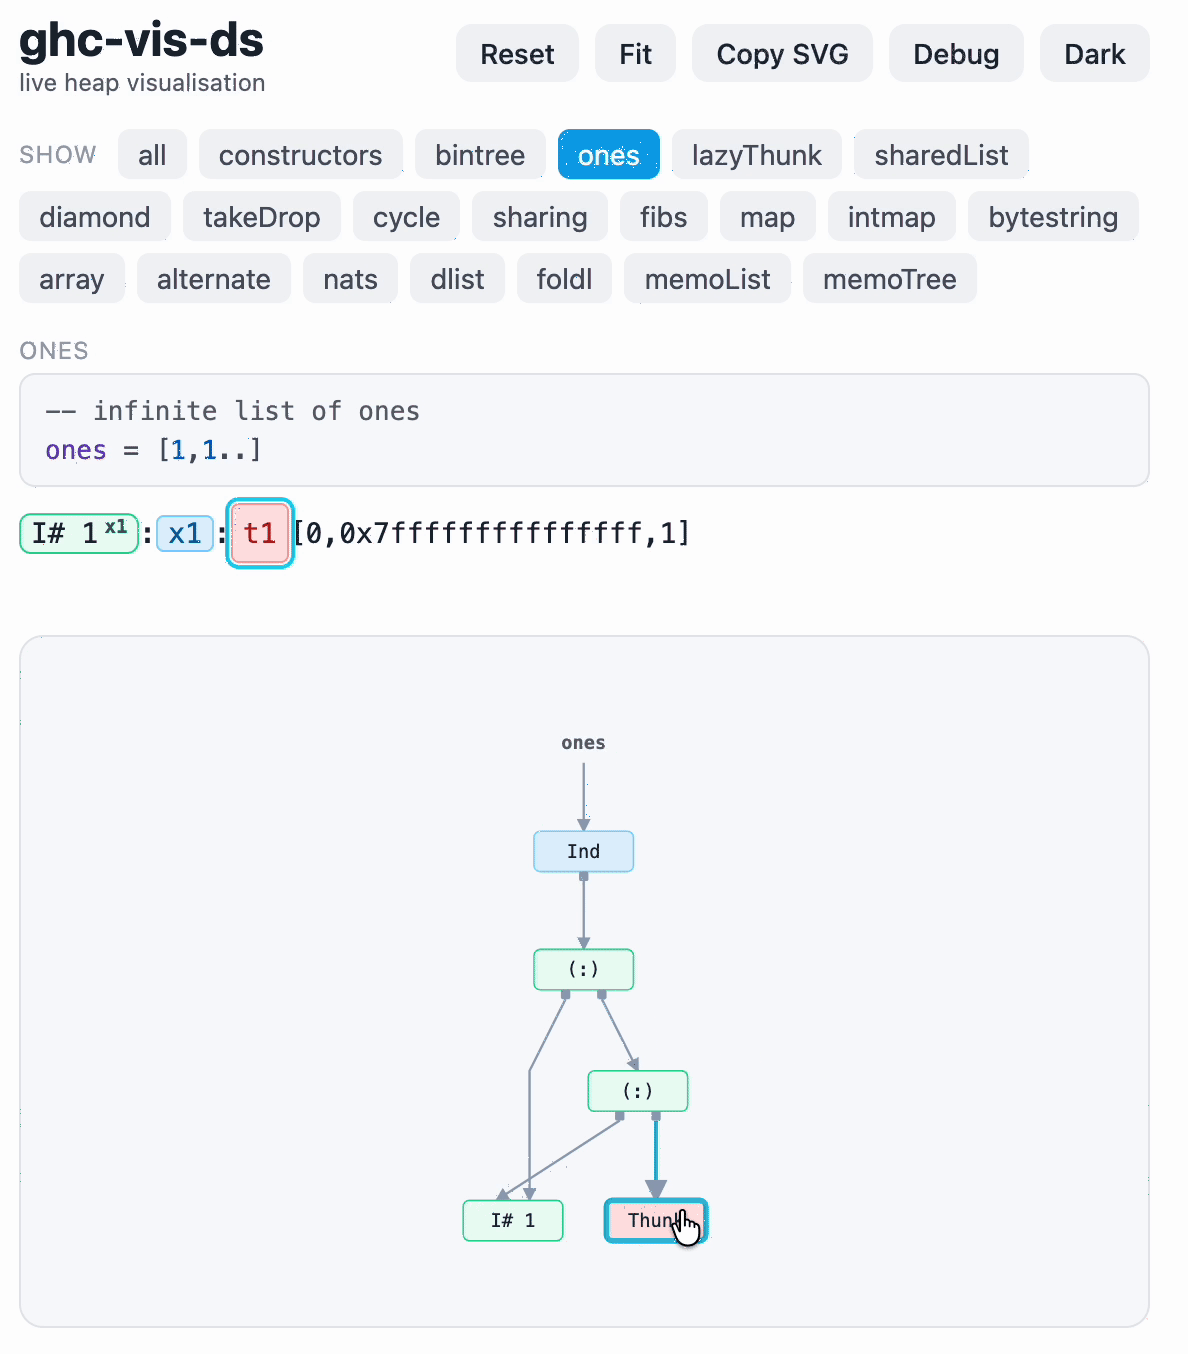
\includegraphics[width=\linewidth,height=0.79\textheight,keepaspectratio]{ghc-vis-ds-ones.png}
    \end{column}
  \end{columns}
\end{frame}

\begin{frame}[fragile]
  \frametitle{Примеры}
  \begin{itemize}
    \item
          \begin{haskell}
            square x = x*x
            square (square (1+1))
          \end{haskell}
          Сколько раз вычислится \haskinline|1+1|?
          \pause
    \item \haskinline|length (take 2 (filter even [1..]))|
          \pause
    \item
          \begin{haskell}
            (&&) :: Bool -> Bool -> Bool
            True  && x = x
            False && x = False
          \end{haskell}
          ведёт себя как в C автоматически.
          \pause
    \item Как определить вариант, который начинает вычисление с правого операнда?
  \end{itemize}
\end{frame}

\begin{frame}[fragile]
  \frametitle{Минусы ленивости}
  \small
  \begin{itemize}
    \item Хранение и обработка отложенных вычислений требуют ресурсов.
    \item Отложенное вычисление может занимать больше памяти, чем результат.
    \item Классический пример:
          \begin{haskellsmall}
            sumAcc [] acc = acc
            sumAcc (x:xs) acc = sumAcc xs (x + acc)

            sumAcc [1..100] 0!$\pause \rightsquigarrow$! sumAcc (1:[2..100]) 0!$\pause \rightsquigarrow$!
            sumAcc [2..100] !$\langle$!1 + 0!$\rangle$!!$\pause \rightsquigarrow$! sumAcc (2:[3..100]) !$\langle$!1 + 0!$\rangle$!!$\pause \rightsquigarrow$!
            sumAcc [3..100] !$\langle$!2 + !$\langle$!1 + 0!$\rangle$!!$\rangle$!!$\pause \rightsquigarrow \ \ldots\ \rightsquigarrow$!
            !$\langle$!100 + ... + !$\langle$!1 + 0!$\rangle$!!$\rangle$!!$\pause \rightsquigarrow $! 5050
          \end{haskellsmall}
    \item \haskinline|sumAcc xs acc = foldl (flip (+)) acc xs|.
          Здесь \haskinline|foldl| копит отложенные сложения. Строгий вариант "--- \haskinline|foldl'|.
  \end{itemize}
\end{frame}

\begin{frame}[fragile]
  \frametitle{Когда ленивость не помогает}
  Что произойдёт в этом примере?
  \begin{haskellsmall}
    length !$\langle$!take 2 !$\langle$!filter (< 2) [1..]!$\rangle$!!$\rangle$! !\onslide<2->! !$\rightsquigarrow$!
    length (1 : !$\langle$!take 1 !$\langle$!filter (< 2) [2..]!$\rangle$!!$\rangle$!) !\onslide<3->! !$\rightsquigarrow$!
    1 + !$\langle$!length !$\langle$!take 1 !$\langle$!filter (< 2) [2..]!$\rangle$!!$\rangle$!!$\rangle$! !\onslide<4->! !$\rightsquigarrow$!
    1 + !$\langle$!length !$\langle$!take 1 !$\langle$!filter (< 2) [3..]!$\rangle$!!$\rangle$!!$\rangle$! !\onslide<5->! !$\rightsquigarrow\ \ldots$! !\onslide<1->!
  \end{haskellsmall}
  \uncover<5->{\small \haskinline|filter| выдаёт \haskinline|1|, но второго элемента не будет: все последующие числа не меньше \haskinline|2|. Поиск продолжается бесконечно; \haskinline|length| не возвращает даже \haskinline|1|.}
\end{frame}

\begin{frame}[fragile,t]
  \frametitle{\haskinline|foldr|: ленивый шаг}
  \begin{itemize}
    \item Запишем \haskinline|map (*2)| через \haskinline|foldr|:
          \begin{haskellsmall}
            step x ys = (x * 2) : ys
          \end{haskellsmall}
  \end{itemize}
    \begin{onlyenv}<1-3>
      \begin{haskellsmall}
        foldr step [] [1..] !\onslide<2->! !$\rightsquigarrow$!
        !$\langle$!1 * 2!$\rangle$! : !$\langle$!foldr step [] [2..]!$\rangle$! !\onslide<1->!
      \end{haskellsmall}
      \uncover<3->{Это уже СЗНФ: \haskinline|(:)| не требует вычисления головы и хвоста.}
    \end{onlyenv}
    \begin{onlyenv}<4->
      Можно потребить только часть результата:
      \begin{haskellsmall}
        sum (take 2 (foldr step [] [1..])) !\onslide<5->! !$\rightsquigarrow$!
        sum (!$\langle$!1 * 2!$\rangle$! : !$\langle$!take 1 !$\langle$!foldr step [] [2..]!$\rangle$!!$\rangle$!) !\onslide<6->! !$\rightsquigarrow$!
        sum [!$\langle$!1 * 2!$\rangle$!, !$\langle$!2 * 2!$\rangle$!] !\onslide<7->! !$\rightsquigarrow$!
        sum [2, 4] !\onslide<8->! !$\rightsquigarrow$! 6 !\onslide<1->!
      \end{haskellsmall}
      \begin{itemize}
        \item<6-> При раскрытии \haskinline|take| произведения остаются отложенными; \haskinline|sum| требует их значения.
        \item<8-> Вызов \haskinline|foldr step [] [3..]| не потребуется.
        \item<9-> А \haskinline|foldr (*) 0 [1..]| не возвращает результат: \haskinline|(*)| требует вычислить рекурсивный результат.
      \end{itemize}
    \end{onlyenv}
\end{frame}

\begin{frame}[fragile]
  \frametitle{Строгие вычисления в Haskell: \haskinline|seq|}
  \begin{itemize}
    \item Мы можем управлять ленивостью явно.
    \item Базовый инструмент для этого: \enquote{волшебная} (её нельзя реализовать на самом Haskell) функция \haskinline|seq :: a -> b -> b|.
          \pause
    \item \haskinline|seq !$e_1$! !$e_2$!| возвращает $e_2$, но требует вычисления $e_1$ до СЗНФ. Порядок вычисления аргументов не гарантируется.
          \pause
    \item Обычно $e_1$ "--- переменная в $e_2$.
    \item Пример использования:
          \begin{haskell*}{escapeinside=||}
            f $! x = seq x (f x)
          \end{haskell*}
    \item Это аналог \haskinline|$|, только вычисляющий аргумент до СЗНФ перед вызовом функции.
  \end{itemize}
\end{frame}

\begin{frame}[fragile]
  \frametitle{Приведение к нормальной форме}
  \small
  \begin{haskellsmall}
    class NFData a where
      rnf :: a -> ()
  \end{haskellsmall}
  \href{https://hackage.haskell.org/package/deepseq/docs/Control-DeepSeq.html#v:rnf}{\haskinline{rnf}} (\emph{reduce to normal form}) приводит аргумент к НФ и возвращает \haskinline|()|. Функцию \haskinline|rnf| приводит лишь к СЗНФ: редексы под лямбдой остаются.
  Для пары: \pause
  \begin{haskellsmall}
    instance (NFData a, NFData b) => NFData (a, b) where
      rnf (x, y) = rnf x `seq` rnf y
  \end{haskellsmall}
  В \href{https://hackage.haskell.org/package/deepseq/docs/Control-DeepSeq.html}{\haskinline{Control.DeepSeq}} через \haskinline|rnf| определены \href{https://hackage.haskell.org/package/deepseq/docs/Control-DeepSeq.html#v:deepseq}{\haskinline{deepseq}} и \href{https://hackage.haskell.org/package/deepseq/docs/Control-DeepSeq.html#v:force}{\haskinline{force}}: \pause
  \begin{haskellsmall}
    deepseq x result = rnf x `seq` result
    force x = x `deepseq` x
  \end{haskellsmall}
  \haskinline|force x| возвращает сам \haskinline|x| после вычисления \haskinline|rnf x|.
\end{frame}

\begin{frame}[fragile]
  \frametitle{Вычисление пары: \haskinline|seq| и \haskinline|deepseq|}
  \small
  Выведем сумму наблюдений. Вычислится ли их число?
  \begin{haskellsmall}
    ghci> let xs = [1..100] :: [Int]
    ghci> let stats = (sum xs, length xs)
    ghci> stats `seq` fst stats
    5050
    ghci> :sprint stats !\pause!
    stats = (5050,_)
  \end{haskellsmall}
  \haskinline|deepseq :: NFData a => a -> b -> b|
  \begin{haskellsmall}
    ghci> import Control.DeepSeq (deepseq, force)
    ghci> stats `deepseq` fst stats  -- или fst (force stats)
    5050
    ghci> :sprint stats !\pause!
    stats = (5050,100)
  \end{haskellsmall}
\end{frame}

\begin{frame}[fragile]
  \frametitle{\haskinline|sumAcc| через \haskinline|seq|}
  \begin{itemize}
    \item Теперь можем определить \haskinline|sumAcc| так:\pause
          \begin{haskell*}{escapeinside=||}
            sumAcc [] acc = acc
            sumAcc (x:xs) acc = sumAcc xs $! x + acc
          \end{haskell*}
    \item Или так:\pause
          \begin{haskell}
            sumAcc [] acc = acc
            sumAcc (x:xs) acc = let a1 = x + acc in
                             a1 `seq` sumAcc xs a1
          \end{haskell}
    \item И процесс вычисления:
          \begin{haskellsmall}
            sumAcc [1..100] 0 !$\rightsquigarrow$! sumAcc (1:[2..100]) 0 !$\pause \rightsquigarrow$!
            let a1 = !$\langle$!1 + 0!$\rangle$! in a1 `seq` sumAcc [2..100] a1 !$\pause \rightsquigarrow$!
            sumAcc [2..100] 1 !$\rightsquigarrow$! sumAcc (2:[3..100]) 1 !$\pause \rightsquigarrow$!
            let a1 = !$\langle$!2 + 1!$\rangle$! in a1 `seq` sumAcc [3..100] a1 !$\pause \rightsquigarrow$!
            !$\rightsquigarrow\ \ldots\ \rightsquigarrow\ $!5050
          \end{haskellsmall}
    \item Заметьте, что список \haskinline|[1..100]| никогда не появляется целиком в памяти!
  \end{itemize}
\end{frame}

\begin{frame}[fragile]
  \frametitle{\haskinline|foldl'|}
  \begin{itemize}
    \item Мы знаем, что сумма списка "--- частный случай свёртки.
    \item Для функций \haskinline|product|, \haskinline|minimum|, \haskinline|maximum| имеем ровно те же проблемы!
    \item Можем определить вариант \haskinline|foldl| (с GHC 9.10 он уже есть в \haskinline|Prelude|):
          \begin{haskellsmall}
            foldl' :: (a -> b -> a) -> a -> [b] -> a
            foldl' f acc []     = acc
            foldl' f acc (x:xs) = acc `seq` foldl' f (f acc x) xs
          \end{haskellsmall}
    \item \pause
          \begin{haskellsmall}
            sum xs = foldl' (+) 0 xs
            product xs = foldl' (*) 1 xs
            minimum xs = foldl1' min xs  -- foldl1' из Data.List
            ...
          \end{haskellsmall}
  \end{itemize}
\end{frame}

\begin{frame}[fragile]
  \frametitle{Среднее: пара в аккумуляторе}
  \small
  \begin{haskellsmall}
    mean :: [Double] -> Double
    mean xs = s' / fromIntegral l'
      where (s', l') = foldl' step (0, 0) xs
            step (s, l) x = (s + x, l + 1)
  \end{haskellsmall}
  \haskinline|foldl'| вычисляет пару до СЗНФ. Что происходит с её полями? \pause
  \begin{haskellsmall}
    foldl' step (0, 0) [1, 2] !$\pause \rightsquigarrow$!
    foldl' step (!$\langle$!0 + 1!$\rangle$!, !$\langle$!0 + 1!$\rangle$!) [2] !$\pause \rightsquigarrow$!
    foldl' step (!$\langle$!!$\langle$!0 + 1!$\rangle$! + 2!$\rangle$!, !$\langle$!!$\langle$!0 + 1!$\rangle$! + 1!$\rangle$!) []
  \end{haskellsmall}
  \pause
  Чтобы избежать этой проблемы, можно вычислить оба поля с помощью \haskinline|force|:
  \begin{haskellsmall}
    step :: (Double, Int) -> Double -> (Double, Int)
    step (s, l) x = let acc = (s + x, l + 1)
                    in force acc
  \end{haskellsmall}
\end{frame}

\begin{frame}[fragile]
  \frametitle{Строгие переменные в образцах}
  \begin{itemize}
    \item Сделаем \haskinline|s| и \haskinline|l| строгими:
          \begin{haskell*}{escapeinside=||}
            step (!s, !l) x = (s + x, l + 1)
          \end{haskell*}
    \item Это превращается в
          \begin{haskell}
            step (s, l) x = s `seq` l `seq` (s + x, l + 1)
          \end{haskell}
          Когда \haskinline|foldl'| требует результат шага, \texttt{!} вычисляет поля предыдущей пары до СЗНФ. Для \haskinline|Double| и \haskinline|Int| это уже НФ: эффект тот же, что у \haskinline|(s, l) `deepseq` (s + x, l + 1)|.
    \item Полные правила перевода \href{https://downloads.haskell.org/~ghc/latest/docs/html/users_guide/exts/strict.html#bang-patterns-informal}{довольно сложные}.
  \end{itemize}
\end{frame}

\begin{frame}[fragile]
  \frametitle{Строгие поля в типах данных}
  \begin{itemize}
    \item Другой способ решить ту же проблему:
          \begin{haskellsmall*}{escapeinside=||}
            data SPair a b = SPair !a !b

            mean :: [Double] -> Double
            mean xs = s' / fromIntegral l'
              where SPair s' l' = foldl' step (SPair 0 0) xs
                    step (SPair s l) x = SPair (s + x) (l + 1)
          \end{haskellsmall*}
          \pause
    \item Восклицательный знак означает, что любое вычисление значения с этим конструктором вычислит и эти поля (до СЗНФ).
    \item То есть конструктор работает как
          \begin{haskell}
            SPair a b = a `seq` b `seq` SPair' a b
          \end{haskell}
          где \haskinline|SPair'| "--- конструктор, который получится без строгих полей.
  \end{itemize}
\end{frame}

\begin{frame}[fragile]
  \frametitle{Дополнительное чтение}
  \begin{itemize}
    \item \href{https://opendsa-server.cs.vt.edu/ODSA/Books/uwosh/cs-331/spring-2020/PL_Book_Spr_2020/html/SLang2ParameterPassing.html}{Parameter-Passing Mechanisms (OpenDSA)}: способы передачи параметров, включая макроподстановку, передачу по имени и по необходимости.
    \item \href{https://blog.acolyer.org/2016/09/14/why-functional-programming-matters/}{Why Functional Programming Matters} (обзор статьи, написанной до появления собственно Haskell)
    \item \href{https://web.archive.org/web/20230322115320/https://www.fpcomplete.com/blog/2017/09/all-about-strictness/}{All About Strictness}
    \item \href{https://apfelmus.nfshost.com/articles/lazy-eval.html}{The Incomplete Guide to Lazy Evaluation}
    \item \href{https://en.wikibooks.org/wiki/Haskell/Laziness}{Laziness в Haskell Wikibook}
  \end{itemize}
\end{frame}


\begin{frame}[fragile]
  \frametitle{Дополнительное чтение: память}
  \begin{itemize}
    \item \href{https://www.plai.org/}{Programming Languages: Application and Interpretation} (бесплатная книга). Глава \emph{Laziness}: как интерпретатор откладывает вычисление и запоминает результат.
    \item \href{https://www.youtube.com/watch?v=I4lnCG18TaY}{Joachim Breitner, Thunks, Sharing, Laziness: The Haskell Heap Visualized}: видеодемонстрация отложенных вычислений, общих ссылок и циклических структур с помощью ghc-vis.
    \item \href{https://haskell.foundation/hs-opt-handbook.github.io/src/Preliminaries/what_makes_fast_hs.html}{The Programs of Consistent Lethargy (Haskell Optimization Handbook)}: ленивость и расход памяти; почему \haskinline|foldl'| не вычисляет поля пары до конца.
  \end{itemize}
\end{frame}

\end{document}
